%%%%%%%%%%%%%%%%%%%%%%%%%%%%%%%%%%%%%%%%%
% Beamer Presentation
% LaTeX Template
% Version 1.0 (10/11/12)
%
% This template has been downloaded from:
% http://www.LaTeXTemplates.com
%
% License:
% CC BY-NC-SA 3.0 (http://creativecommons.org/licenses/by-nc-sa/3.0/)
%
%%%%%%%%%%%%%%%%%%%%%%%%%%%%%%%%%%%%%%%%%

%----------------------------------------------------------------------------------------
%	PACKAGES AND THEMES
%----------------------------------------------------------------------------------------

\documentclass[UTF8,aspectratio=169,14pt]{ctexbeamer}

\usepackage{hyperref}
\hypersetup{
	colorlinks=true,
	linkcolor=red,
	anchorcolor=blue,
	citecolor=green
}

\mode<presentation> {
	
	% The Beamer class comes with a number of default slide themes
	% which change the colors and layouts of slides. Below this is a list
	% of all the themes, uncomment each in turn to see what they look like.
	
	%\usetheme{default}
	%\usetheme{AnnArbor}
	%\usetheme{Antibes}
	%\usetheme{Bergen}
	%\usetheme{Berkeley}
	%\usetheme{Berlin}
	%\usetheme{Boadilla}
	%\usetheme{CambridgeUS}
	%\usetheme{Copenhagen}
	%\usetheme{Darmstadt}
	%\usetheme{Dresden}
	%\usetheme{Frankfurt}
	%\usetheme{Goettingen}
	%\usetheme{Hannover}
	%\usetheme{Ilmenau}
	%\usetheme{JuanLesPins}
	%\usetheme{Luebeck}
	\usetheme{Madrid}
	%\usetheme{Malmoe}
	%\usetheme{Marburg}
	%\usetheme{Montpellier}
	%\usetheme{PaloAlto}
	%\usetheme{Pittsburgh}
	%\usetheme{Rochester}
	%\usetheme{Singapore}
	%\usetheme{Szeged}
	%\usetheme{Warsaw}
	
	% As well as themes, the Beamer class has a number of color themes
	% for any slide theme. Uncomment each of these in turn to see how it
	% changes the colors of your current slide theme.
	
	%\usecolortheme{albatross}
	%\usecolortheme{beaver}
	%\usecolortheme{beetle}
	%\usecolortheme{crane}
	%\usecolortheme{dolphin}
	%\usecolortheme{dove}
	%\usecolortheme{fly}
	%\usecolortheme{lily}
	%\usecolortheme{orchid}
	%\usecolortheme{rose}
	%\usecolortheme{seagull}
	%\usecolortheme{seahorse}
	%\usecolortheme{whale}
	%\usecolortheme{wolverine}
	
	%\setbeamertemplate{footline} % To remove the footer line in all slides uncomment this line
	%\setbeamertemplate{footline}[page number] % To replace the footer line in all slides with a simple slide count uncomment this line
	
	%\setbeamertemplate{navigation symbols}{} % To remove the navigation symbols from the bottom of all slides uncomment this line
}

\usepackage{graphicx} % Allows including images
\graphicspath{{./figs/}}
\usepackage{booktabs} % Allows the use of \toprule, \midrule and \bottomrule in tables
\usepackage{longtable}
\usepackage{listings}
\usepackage{xcolor}
\lstset{numbers=left, %设置行号位置
	numberstyle=\tiny, %设置行号大小
	keywordstyle=\color{blue}, %设置关键字颜色
	commentstyle=\color[cmyk]{1,0,1,0}, %设置注释颜色
	frame=single, %设置边框格式
	escapeinside=``, %逃逸字符(1左面的键),用于显示中文
	%breaklines, %自动折行
	extendedchars=false, %解决代码跨页时,章节标题,页眉等汉字不显示的问题
	xleftmargin=2em,xrightmargin=2em, aboveskip=1em, %设置边距
	tabsize=4, %设置tab空格数
	showspaces=false %不显示空格
}
% Fonts
% \usepackage{libertine}
% \setmonofont{Courier}
\setCJKsansfont[ItalicFont=Noto Serif CJK SC Black, BoldFont=Noto Sans CJK SC Black]{Noto Sans CJK SC}


%----------------------------------------------------------------------------------------
% TITLE PAGE
%----------------------------------------------------------------------------------------

\title[第18讲]{第十八讲 :文件系统实例} % The short title appears at the bottom of every slide, the full title is only on the title page
\subtitle{第3节:EXT4文件系统}
\author{向勇、陈渝、李国良} % Your name
\institute[清华大学] % Your institution as it will appear on the bottom of every slide, may be shorthand to save space
{
  清华大学计算机系 \\ % Your institution for the title page
  \medskip
  \textit{xyong,yuchen,liguoliang@tsinghua.edu.cn} % Your email address
}
\date{\today} % Date, can be changed to a custom date

\begin{document}

\begin{frame}
\titlepage % Print the title page as the first slide
\end{frame}

%----------------------------------------------
%\begin{frame}
%\frametitle{提纲} % Table of contents slide, comment this block out to remove it
%\tableofcontents % Throughout your presentation, if you choose to use \section{} and \subsection{} commands, these will automatically be printed on this slide as an overview of your presentation
%
%\end{frame}
%----------------------------------------------
%%  PRESENTATION SLIDES
%----------------------------------------------
\section{第3节:EXT4文件系统} % Sections can be created in order to organize your presentation into discrete blocks, all sections and subsections are automatically printed in the table of contents as an overview of the talk
%----------------------------------------------
%\subsection{EXT4 } % A subsection can be created just before a set of slides with a common theme to further break down your presentation into chunks
%----------------------------------------------
\begin{frame}
\frametitle{提纲} % Table of contents slide, comment this block out to remove it
\tableofcontents % Throughout your presentation, if you choose to use \section{} and \subsection{} commands, these will automatically be printed on this slide as an overview of your presentation
\end{frame}
%------------------------------------------------
\subsection{历史}
\begin{frame}[plain]
    \frametitle{历史}
%    \framesubtitle{xxxx}
% from https://opensource.com/article/17/5/introduction-ext4-filesystem

	\frametitle{ }
	\begin{columns}
		\begin{column}{.45\textwidth}
	    
\includegraphics[width=0.6\textwidth]{minix}
	    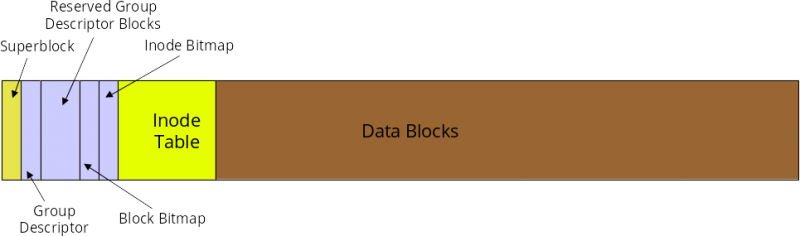
\includegraphics[width=0.8\textwidth]{ext-fs-layout}
	    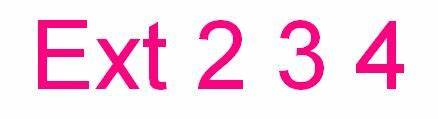
\includegraphics[width=0.6\textwidth]{ext2-3-4}
		
\includegraphics[width=0.6\textwidth]{ext4-logo}	
			
		\end{column}
		
		\begin{column}{.5\textwidth}
		  	\begin{block}{Linux文件系统历史}
		  	EXT[1-4]文件系统家族是为Linux编写的。但它来源于1987年首次发布的Minix操作系统和Minix文件系统。从Minix开始回顾EXT文件系统家族历史和技术,更容易了解EXT4文件系统。
		  \end{block}

		\end{column}
	\end{columns}
\tiny Reference: \\
OSTEP txtbook: Crash Consistency: FSCK and Journaling; Ext4 slides from Mingming Cao; An introduction to Linux's EXT4 filesystem by  David Both

\end{frame}



%----------------------------------------------
\begin{frame}[fragile]
	\frametitle{历史:MINIX FS}
	%    \framesubtitle{xxxx}
	% from https://opensource.com/article/17/5/introduction-ext4-filesystem
	
	\frametitle{ }
	\begin{columns}[t]
		\begin{column}{.4\textwidth}
			
\includegraphics[width=0.6\textwidth]{minix}
			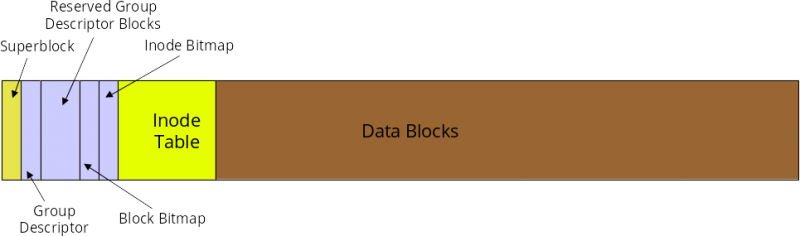
\includegraphics[width=0.8\textwidth]{ext-fs-layout}
	
			\begin{itemize}
				\item Linus Torvalds开始编写Linux内核时就需要一个文件系统。
				\item 拿来主义:直接采用Andrew S. Tanenbaum编写Minix文件系统
			\end{itemize}
		
		\end{column} \pause
		
		\begin{column}{.6\textwidth}			
			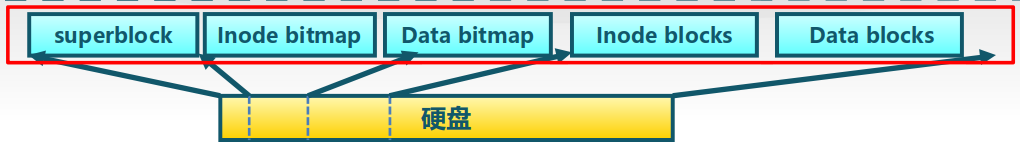
\includegraphics[width=1.\textwidth]{minix-layout}
			MINIX FS
				\begin{itemize}
					\item 引导扇区:在其上安装了硬盘的第一个扇区。引导块包括一个很小的引导记录和一个分区表。
					\item 超级块:每个分区中的第一个块是一个超级块,其中包含元数据,该元数据定义了其他文件系统结构,并将它们定位在分配给该分区的物理磁盘上。
%					\item 索引节点区位图:表明哪些索引节点已使用和哪些索引节点空闲。
%					\item 索引节点区:它在磁盘上有自己的空间。每个inode包含有关一个文件的信息,包括数据块的位置,即属于该文件的区域。
%					\item 数据区位图:来跟踪使用和免费的数据区。
%					\item 数据区:保存实际存储数据。
				\end{itemize}
			
		\end{column}
	\end{columns}
	
\end{frame}

%----------------------------------------------
\begin{frame}[fragile]
	\frametitle{历史:MINIX FS}
	%    \framesubtitle{xxxx}
	% from https://opensource.com/article/17/5/introduction-ext4-filesystem
	
	\frametitle{ }
	\begin{columns}[t]
		\begin{column}{.4\textwidth}
			
\includegraphics[width=0.6\textwidth]{minix}
			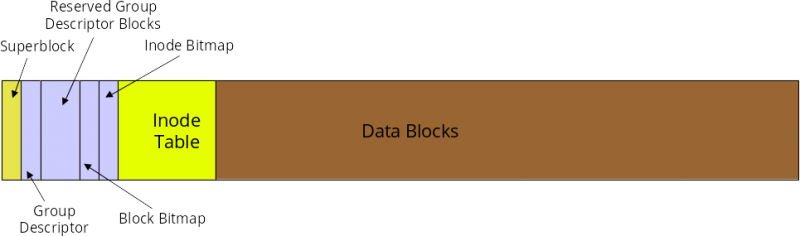
\includegraphics[width=0.8\textwidth]{ext-fs-layout}
			
			\begin{itemize}
				\item Linus Torvalds在编写原始的Linux内核时,他需要一个文件系统,但是不想编写一个文件系统。
				\item 拿来主义:直接采用Andrew S. Tanenbaum编写Minix文件系统
			\end{itemize}
			
		\end{column}
		
		\begin{column}{.6\textwidth}			
			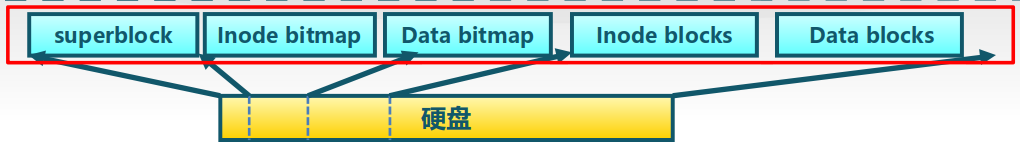
\includegraphics[width=1.\textwidth]{minix-layout}
			MINIX FS
			\begin{itemize}
%				\item 引导扇区:在其上安装了硬盘的第一个扇区。引导块包括一个很小的引导记录和一个分区表。
%				\item 超级块:每个分区中的第一个块是一个超级块,其中包含元数据,该元数据定义了其他文件系统结构,并将它们定位在分配给该分区的物理磁盘上。
				\item 索引节点区位图:表明哪些索引节点已使用和哪些索引节点空闲。
				\item 索引节点区:它在磁盘上有自己的空间。每个inode包含有关一个文件的信息,包括数据块的位置,即属于该文件的区域。
				\item 数据区位图:来跟踪使用和空闲的数据区。
				\item 数据区:保存实际存储数据。
			\end{itemize}
			
		\end{column}
	\end{columns}
	
\end{frame}


%----------------------------------------------
\begin{frame}[fragile]
	\frametitle{历史:EXT FS}
	%    \framesubtitle{xxxx}
	% from https://opensource.com/article/17/5/introduction-ext4-filesystem
	
	\frametitle{ }
	\begin{columns}[t]
		\begin{column}{.35\textwidth}

			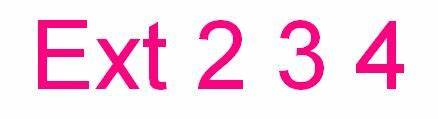
\includegraphics[width=0.5\textwidth]{ext2-3-4}
%			
\includegraphics[width=0.4\textwidth]{ext4-logo}
			\begin{itemize}
				\item 最初的EXT文件系统(扩展)由RémyCard编写
				\item 1992年随Linux发行
				\item 克服Minix文件系统的某些大小限制
				
			\end{itemize}
			
		\end{column}
		
		\begin{column}{.7\textwidth}			
			EXT FS
			\begin{itemize}
				\item 主要的结构更改是基于Unix文件系统(UFS)(也称为Berkeley快速文件系统(FFS))的文件系统的元数据。
				\item 因为存在重大问题,很快被EXT2文件系统所取代,也很少有关于EXT文件系统的公开信息
			\end{itemize}
			
		\end{column}
	\end{columns}
	
\end{frame}


%----------------------------------------------
\begin{frame}[fragile]
	\frametitle{历史:EXT2}
	%    \framesubtitle{xxxx}
	% from https://opensource.com/article/17/5/introduction-ext4-filesystem
	
	\frametitle{ }
	\begin{columns}[t]
		\begin{column}{.3\textwidth}
			
			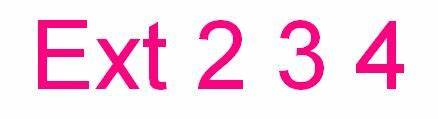
\includegraphics[width=0.5\textwidth]{ext2-3-4}
			%			
\includegraphics[width=0.4\textwidth]{ext4-logo}
			\begin{itemize}
				\item EXT2文件系统具有与EXT基本相同的元数据结构
				\item 稳定可靠性有很大提升
				\item 被广泛使用于Linux的早期版本。
				
			\end{itemize}
			
		\end{column}
		
		\begin{column}{.7\textwidth}			
			EXT2 FS
			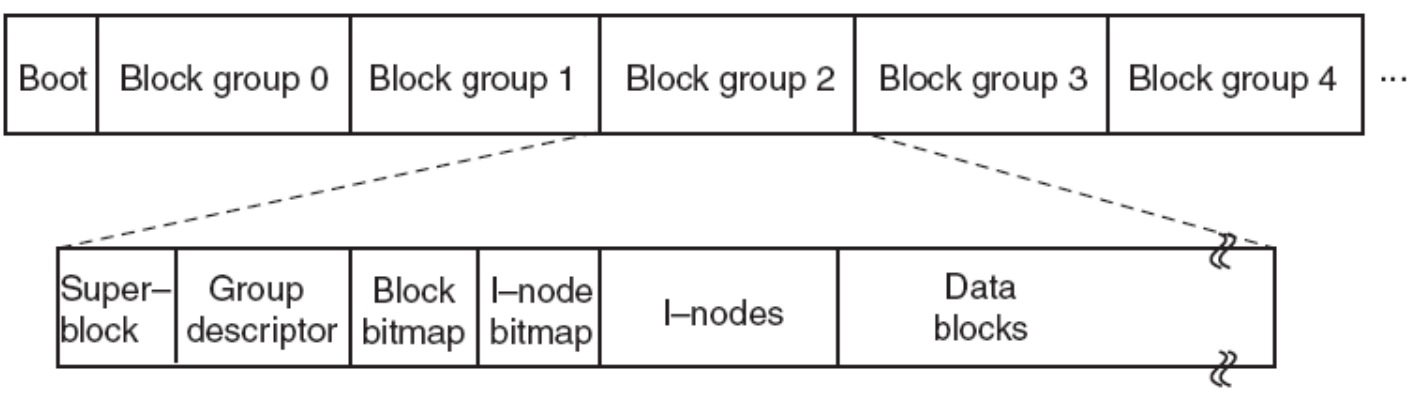
\includegraphics[width=1.\textwidth]{ext2-layout}
			\begin{itemize}
				\item 同一目录的文件存储在同一个block group中
				\item 不同目录的文件分布在不同的block group中
				\item 掉电或死机后,文件系统恢复正常要花费很长时间
			\end{itemize}
			
		\end{column}
	\end{columns}
	
\end{frame}



%----------------------------------------------
\begin{frame}[fragile]
	\frametitle{历史:EXT3}
	%    \framesubtitle{xxxx}
	% from https://opensource.com/article/17/5/introduction-ext4-filesystem
	
	\frametitle{ }
	\begin{columns}[t]
		\begin{column}{.4\textwidth}
			
			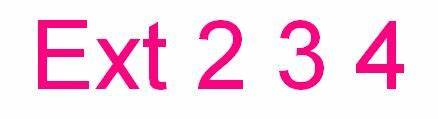
\includegraphics[width=0.5\textwidth]{ext2-3-4}
			%			
\includegraphics[width=0.4\textwidth]{ext4-logo}
			\begin{itemize}
				\item 目标:减少异常文件系统的恢复时间
				\item EXT3文件系统增加了journal机制,预先记录将对文件系统执行的更改。
				\item 其余磁盘结构与EXT2中的相同。
				
			\end{itemize}
			
		\end{column}
		
		\begin{column}{.5\textwidth}			
			EXT3 FS
			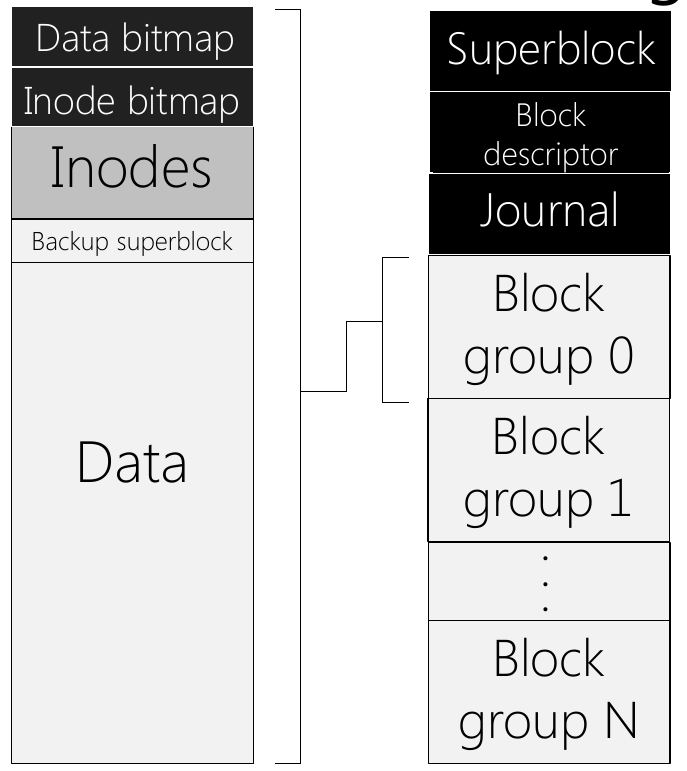
\includegraphics[width=.8\textwidth]{ext3-layout}
			
		\end{column}
	\end{columns}
	
\end{frame}


%----------------------------------------------
\begin{frame}[fragile]
	\frametitle{历史:EXT4}
	%    \framesubtitle{xxxx}
	% from https://opensource.com/article/17/5/introduction-ext4-filesystem
	
	\frametitle{ }
	\begin{columns}[t]
		\begin{column}{.3\textwidth}
			
			
\includegraphics[width=0.5\textwidth]{ext4-logo}
			%			
\includegraphics[width=0.4\textwidth]{ext4-logo}
			\begin{itemize}
				\item EXT4文件系统进一步改善了性能,可靠性和大容量支持
				
			\end{itemize}
			
		\end{column}
		
		\begin{column}{.7\textwidth}			
			EXT4 FS
			\begin{itemize}
				\item 可靠性:添加了元数据和日志校验和
				\item 文件系统时间戳:为满足关键任务要求,改进了文件系统时间戳,增加了纳秒精度时间间隔
				\item 性能:为提高容量和大容量文件访问性能,把数据分配从固定块更改为扩展区
			\end{itemize}
			
		\end{column}
	\end{columns}
	
\end{frame}


%----------------------------------------------
\begin{frame}[fragile]
	\frametitle{历史:EXT4}
	%    \framesubtitle{xxxx}
	%% figure
	\begin{figure}
		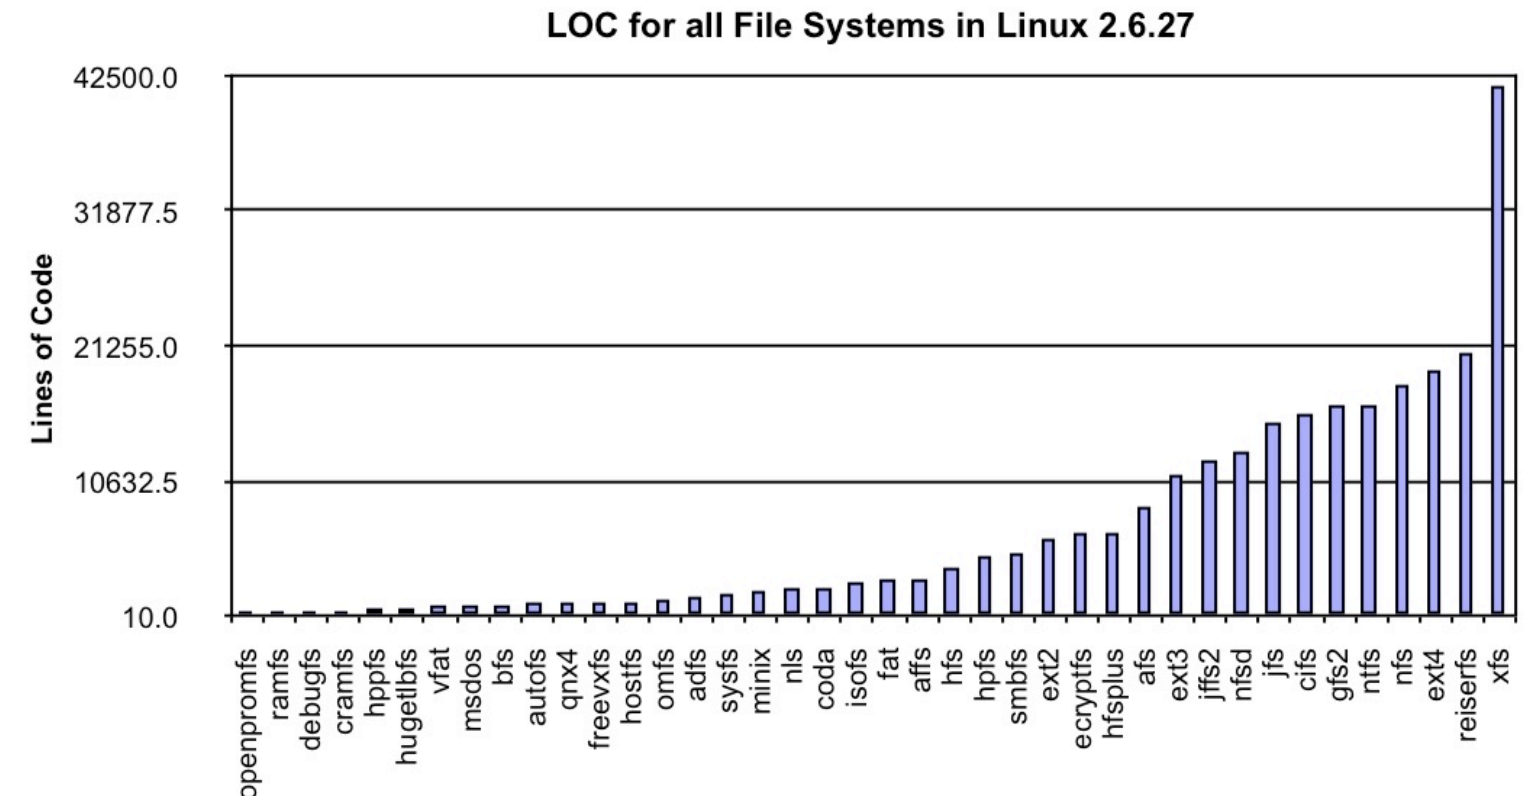
\includegraphics[width=0.93\linewidth]{linux-allfs}
		% \caption{xxxx}
	\end{figure}

\end{frame}



%----------------------------------------------
\begin{frame}
\frametitle{提纲} % Table of contents slide, comment this block out to remove it
\tableofcontents % Throughout your presentation, if you choose to use \section{} and \subsection{} commands, these will automatically be printed on this slide as an overview of your presentation
\end{frame}
%------------------------------------------------
\subsection{支持大容量存储}
\begin{frame}[fragile]
	\frametitle{细节 -- 支持大容量存储}
	%    \framesubtitle{xxxx}
	% from https://opensource.com/article/17/5/introduction-ext4-filesystem
	
	\frametitle{ }
	\begin{columns}[t]
		\begin{column}{.3\textwidth}
			
			
\includegraphics[width=0.5\textwidth]{ext4-logo}
			%			
\includegraphics[width=0.4\textwidth]{ext4-logo}
			\begin{itemize}
				\item EXT4的重要特征:支持大容量存储和快速恢复异常状态
				
			\end{itemize}
			
		\end{column}
		
		\begin{column}{.7\textwidth}			
			EXT4 FS: 支持大容量存储
			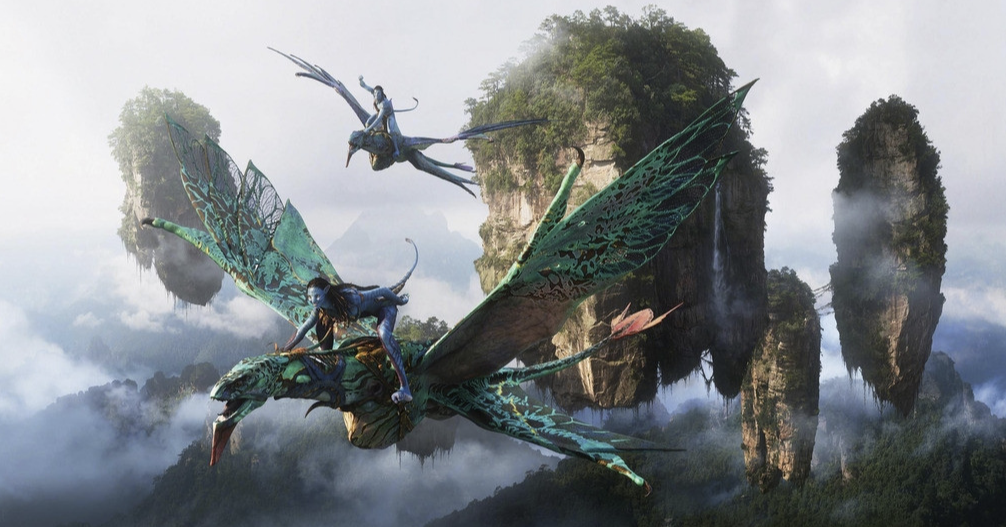
\includegraphics[width=.8\textwidth]{avatar}
			\begin{itemize}
				\item 一部蓝光 8K 3D电影,512GB~1TB
				\item 1EB($2^{60}$) 文件系统大小,16TB 文件大小,子目录个数无限制
			\end{itemize}
			
		\end{column}
	\end{columns}
	
\end{frame}


%----------------------------------------------
\begin{frame}[fragile]
	\frametitle{细节 -- 支持大容量存储}
	%    \framesubtitle{xxxx}
	% from https://opensource.com/article/17/5/introduction-ext4-filesystem
	\centering
    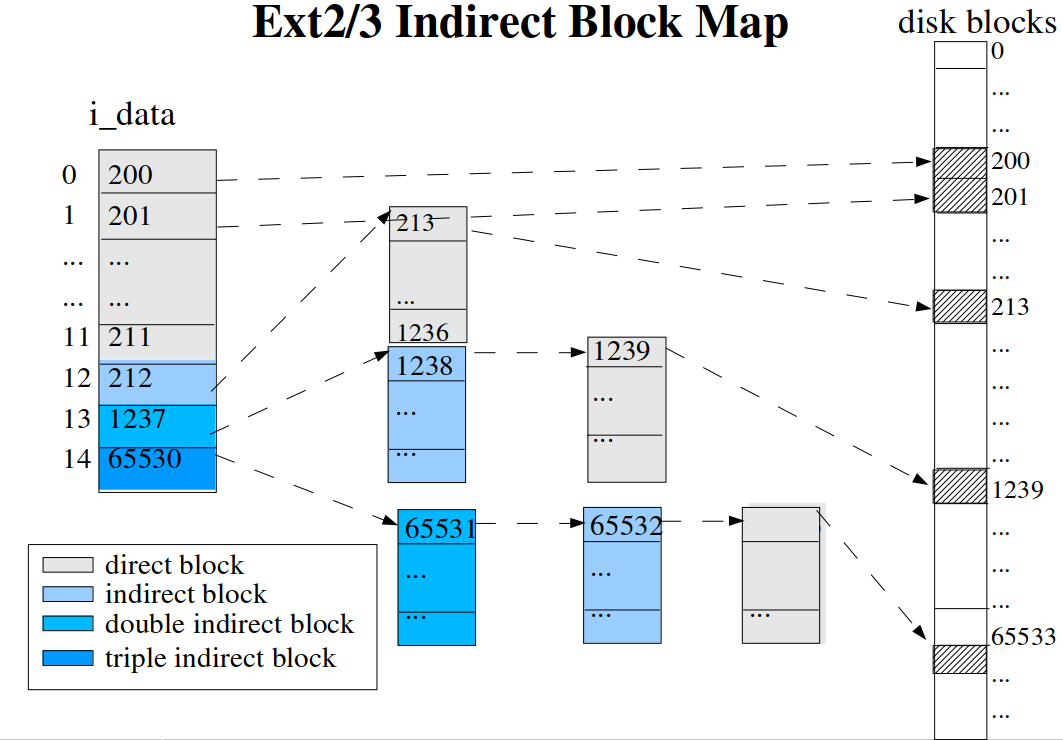
\includegraphics[width=.68\textwidth]{ext2-3-indirect-block}
	
\end{frame}

%----------------------------------------------
\begin{frame}[fragile]
	\frametitle{细节 -- 支持大容量存储}
	%    \framesubtitle{xxxx}
	% from https://opensource.com/article/17/5/introduction-ext4-filesystem
%		\centering
		\Large
	extent: 一段连续的储存块
\centering
	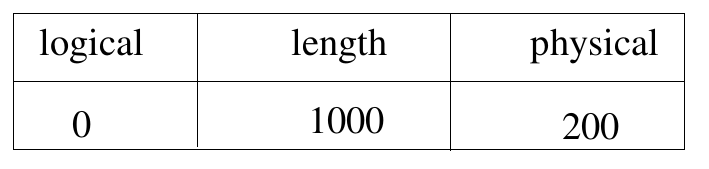
\includegraphics[width=.6\textwidth]{ext4-extent-format}
	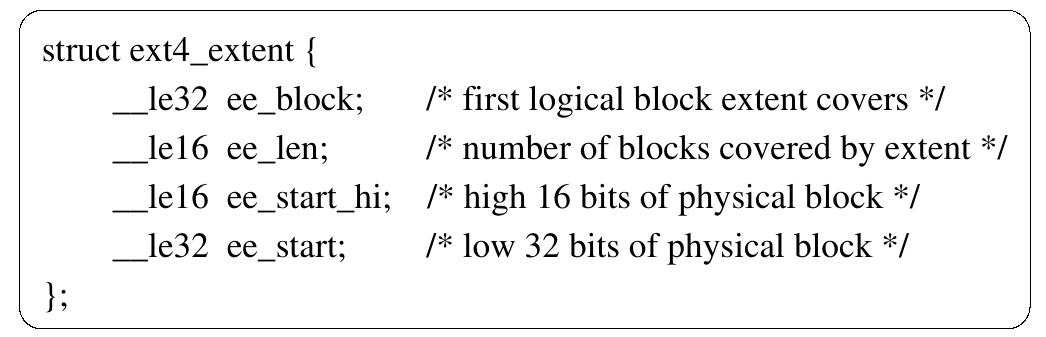
\includegraphics[width=.6\textwidth]{ext4-extent-struct}
\end{frame}


%----------------------------------------------
\begin{frame}[fragile]
	\frametitle{细节 -- 支持大容量存储}
	%    \framesubtitle{xxxx}
	% from https://opensource.com/article/17/5/introduction-ext4-filesystem
	%		\centering
	\begin{columns}
	\begin{column}{.4\textwidth}
		
	extent: 一段连续的储存块
\centering
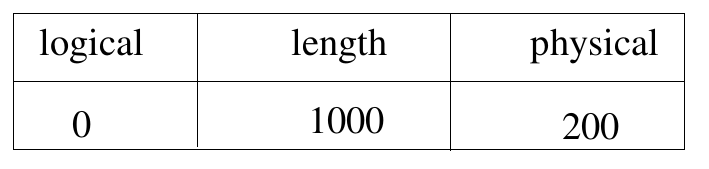
\includegraphics[width=.8\textwidth]{ext4-extent-format}
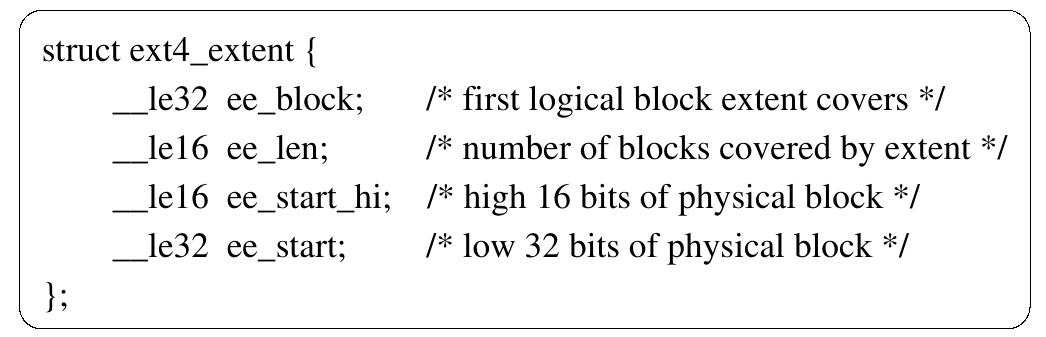
\includegraphics[width=.8\textwidth]{ext4-extent-struct}
		
	\end{column}
	
		\begin{column}{.6\textwidth}			

	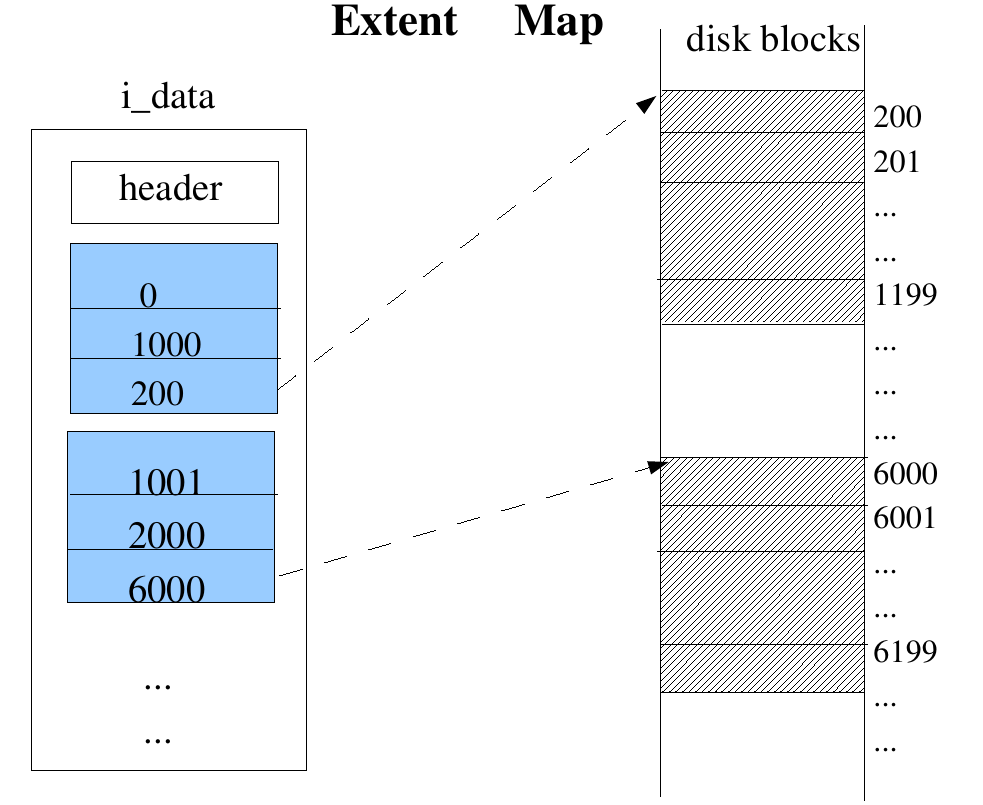
\includegraphics[width=.9\textwidth]{ext4-extent-map}

	
\end{column}
\end{columns}

\end{frame}


%----------------------------------------------
\begin{frame}[fragile]
	\frametitle{细节 -- 支持大容量存储}
	%    \framesubtitle{xxxx}
	% from https://opensource.com/article/17/5/introduction-ext4-filesystem
	%		\centering
%	\Large
%	extent: 一段连续的储存块
	\centering
	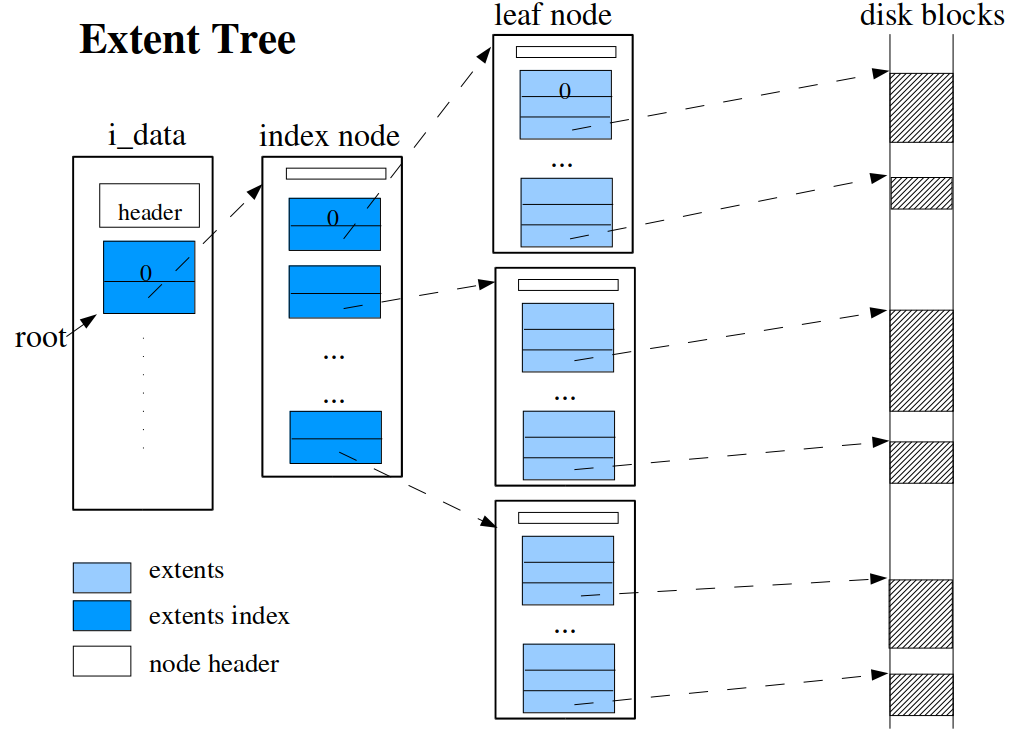
\includegraphics[width=.6\textwidth]{ext4-extent-tree}

\end{frame}




%----------------------------------------------
\begin{frame}
\frametitle{提纲} % Table of contents slide, comment this block out to remove it
\tableofcontents % Throughout your presentation, if you choose to use \section{} and \subsection{} commands, these will automatically be printed on this slide as an overview of your presentation
\end{frame}
%------------------------------------------------
\subsection{支持异常恢复}
\begin{frame}[fragile]
	\frametitle{细节 -- 支持恢复异常}
	%    \framesubtitle{xxxx}
	% from https://opensource.com/article/17/5/introduction-ext4-filesystem
	%		\centering
	%	\Large
	EXT4: 恢复异常文件系统 for crash-consistency problem
	
	\centering
	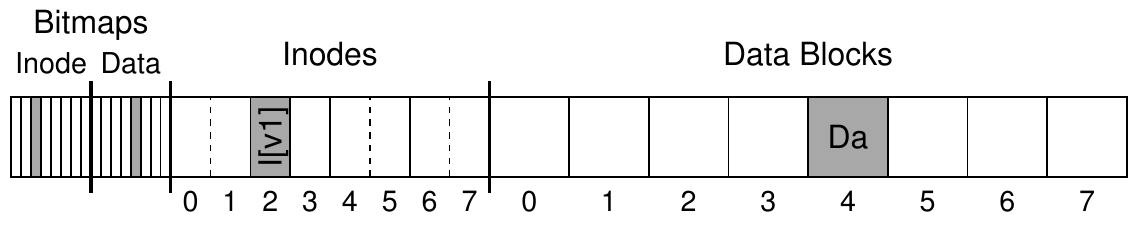
\includegraphics[width=1.\textwidth]{crash-ex}
	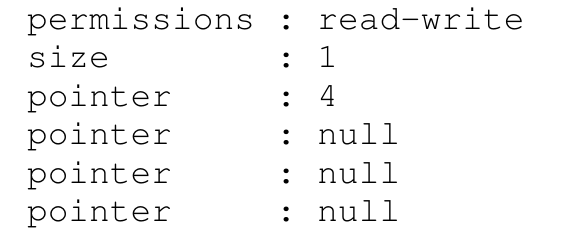
\includegraphics[width=.5\textwidth]{crash-ex-iv1}
\end{frame}


%----------------------------------------------
\begin{frame}[fragile]
	\frametitle{细节 -- 支持恢复异常}
	%    \framesubtitle{xxxx}
	% from https://opensource.com/article/17/5/introduction-ext4-filesystem
	%		\centering
	%	\Large
	EXT4: 恢复异常文件系统 for crash-consistency problem
	
	\centering
	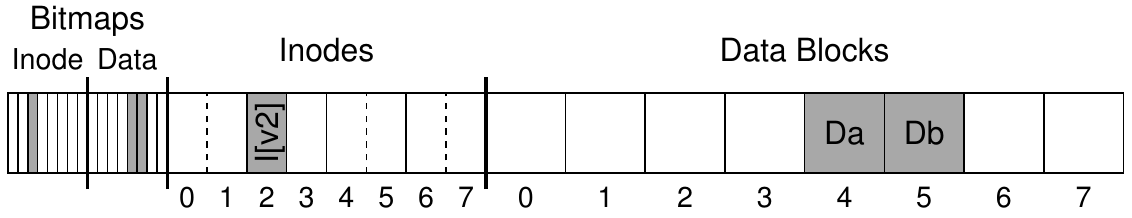
\includegraphics[width=1.\textwidth]{crash-ex-ver2}
	
	
		\begin{columns}
		\begin{column}{.5\textwidth}
			
		
			\centering
	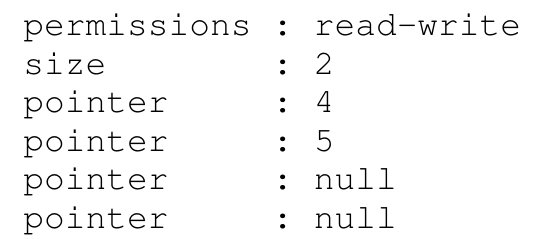
\includegraphics[width=1.\textwidth]{crash-ex-iv2}
			
		\end{column}
		\pause
		\begin{column}{.5\textwidth}			
		3个写操作
		\begin{itemize}
	\item inode (I[v2]) 
	\item bitmap (B[v2])
	\item data block (Db)
\end{itemize}
			
		\end{column}
	\end{columns}
	
\end{frame}



%----------------------------------------------
\begin{frame}[fragile]
	\frametitle{细节 -- 支持恢复异常 -- Crash 场景}
	%    \framesubtitle{xxxx}
	% from https://opensource.com/article/17/5/introduction-ext4-filesystem
	%		\centering
	%	\Large
	\begin{columns}
	\begin{column}{.4\textwidth}
	EXT4: 恢复异常文件系统 for crash-consistency problem
	
	\centering
	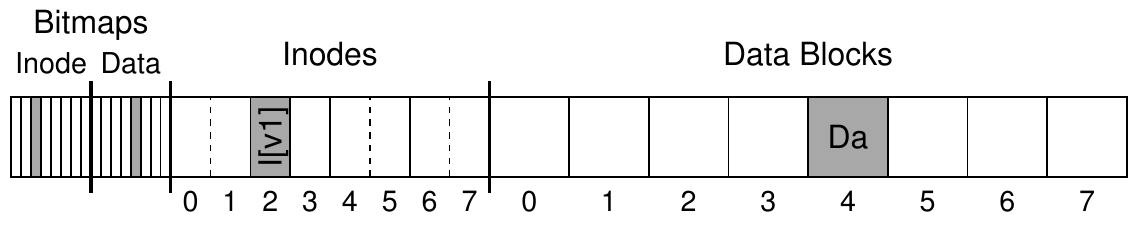
\includegraphics[width=1.\textwidth]{crash-ex}
	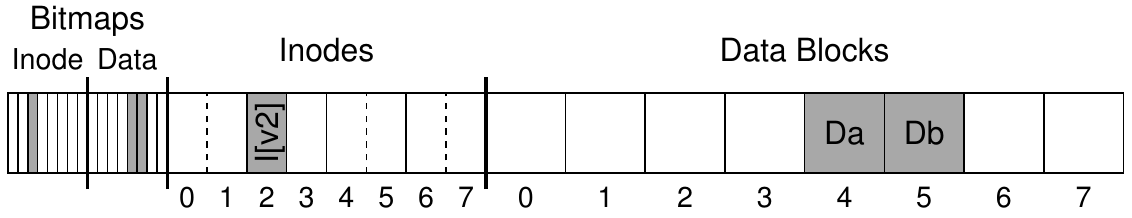
\includegraphics[width=1.\textwidth]{crash-ex-ver2}
%	\centering
	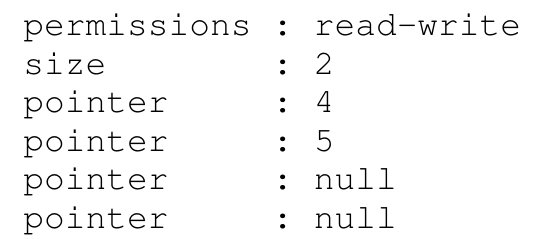
\includegraphics[width=.8\textwidth]{crash-ex-iv2}	
	\end{column}
	\pause
	\begin{column}{.6\textwidth}			
			Crash 场景
			\begin{itemize}
				\item 只有data block (Db) 写入磁盘
				\item 只有 inode (I[v2])  写入磁盘
				\item 只有 bitmap (B[v2])  写入磁盘
				\pause
				\item inode(I[v2]) 和 bitmap (B[v2])写入磁盘
				\item inode(I[v2])和 data block(Db)写入磁盘
				\item bitmap(B[v2])和 data block(Db)写入磁盘
			\end{itemize}
			
		\end{column}
	\end{columns}
	
\end{frame}


%----------------------------------------------
\begin{frame}[fragile]
	\frametitle{细节 -- 支持恢复异常 -- FSCK}
	%    \framesubtitle{xxxx}
	% from https://opensource.com/article/17/5/introduction-ext4-filesystem
	%		\centering
	%	\Large
	\begin{columns}
		\begin{column}{.4\textwidth}
			EXT4: 恢复异常文件系统 for crash-consistency problem
			
			\centering
			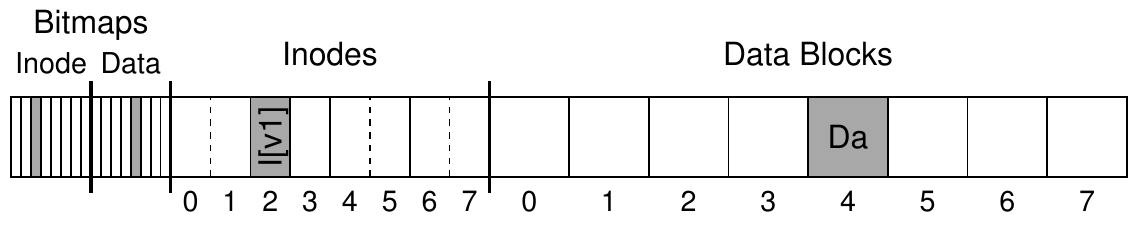
\includegraphics[width=1.\textwidth]{crash-ex}
			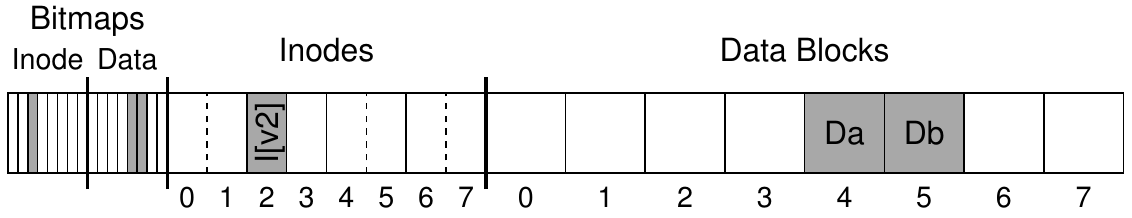
\includegraphics[width=1.\textwidth]{crash-ex-ver2}
			%	\centering
			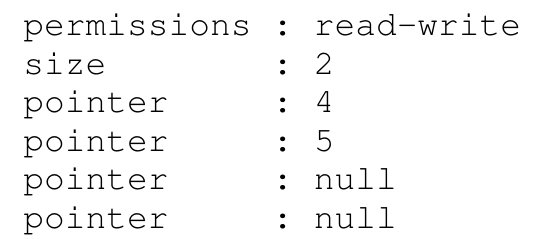
\includegraphics[width=.8\textwidth]{crash-ex-iv2}	
		\end{column}
%		\pause
		\begin{column}{.6\textwidth}			
			解决方法1 : File System Checker (fsck)
			\begin{itemize}
				\item Superblock:文件系统大小大于已分配的块数 \pause
				\item Free blocks: bitmap v.s. Free blocks \pause
				\item Inode state/links:有效的类型字段/链接计数 \pause
				\item Duplicates:两个inode指向同一data  \pause
				\item Bad blocks:指针显然指向超出其有效范围 \pause
				\item Directory:“.”和“..”是头两项
			\end{itemize}
			\pause
			\Large 太慢
		\end{column}
	\end{columns}
	
\end{frame}

%----------------------------------------------
\begin{frame}[fragile]
	\frametitle{细节 -- 支持恢复异常 -- Journaling}
	%    \framesubtitle{xxxx}
	% from https://opensource.com/article/17/5/introduction-ext4-filesystem
	%		\centering
	%	\Large
	\begin{columns}
		\begin{column}{.4\textwidth}
			EXT4: 恢复异常文件系统 for crash-consistency problem
			
			\centering
			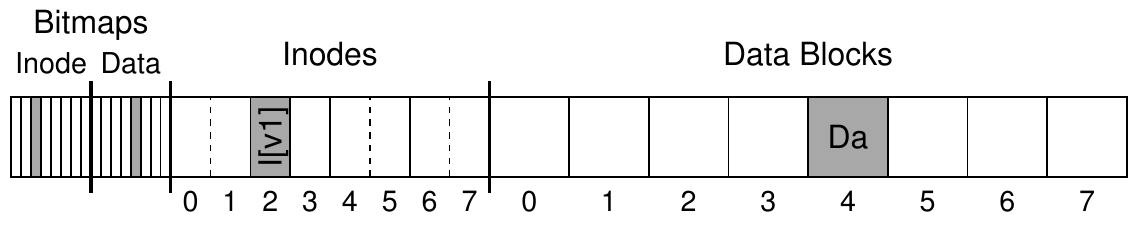
\includegraphics[width=1.\textwidth]{crash-ex}
			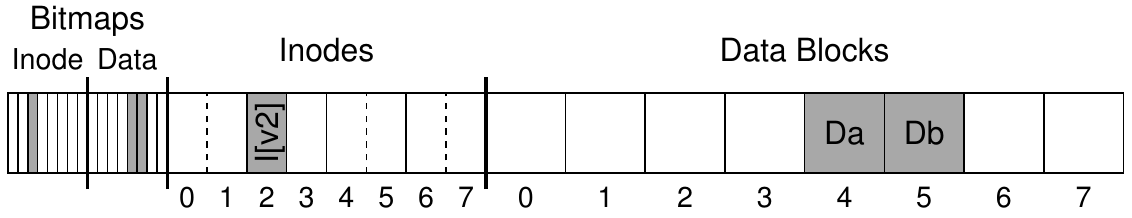
\includegraphics[width=1.\textwidth]{crash-ex-ver2}
			%	\centering
			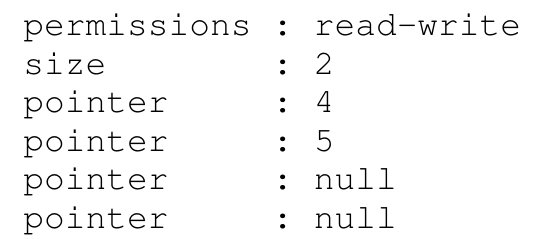
\includegraphics[width=.8\textwidth]{crash-ex-iv2}	
		\end{column}
		%		\pause
		\begin{column}{.6\textwidth}			
			解决方法2 : 日志 Journaling (Write-Ahead Logging)
			\begin{itemize}
				\item 从数据库管理系统的世界中窃取一个想法
				\item 最早(1987)在Cedar文件系统中出现
				\item 在EXT3/4,JFS,XFS,NTFS等应用
			\end{itemize}
			\pause
			基本思路
			\begin{itemize}	
				\item 更新磁盘时,在覆盖相关结构之前,先写下一点日志(在磁盘上某个设定好的其他位置),以描述要执行的操作。
			\end{itemize}

		\end{column}
	\end{columns}
	
\end{frame}


%----------------------------------------------
\begin{frame}[fragile]
	\frametitle{细节 -- 支持恢复异常 -- Data Journaling}
	%    \framesubtitle{xxxx}
	% from https://opensource.com/article/17/5/introduction-ext4-filesystem
	%		\centering
	%	\Large
	\begin{columns}
		\begin{column}{.5\textwidth}
			EXT4: 恢复异常文件系统 for crash-consistency problem
			
			\centering
			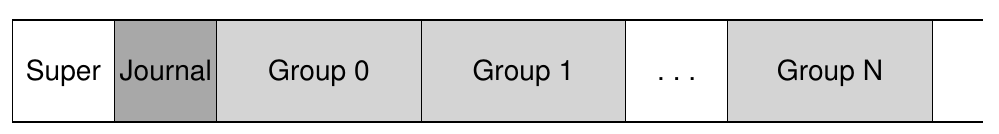
\includegraphics[width=1.\textwidth]{ext3-journal}
			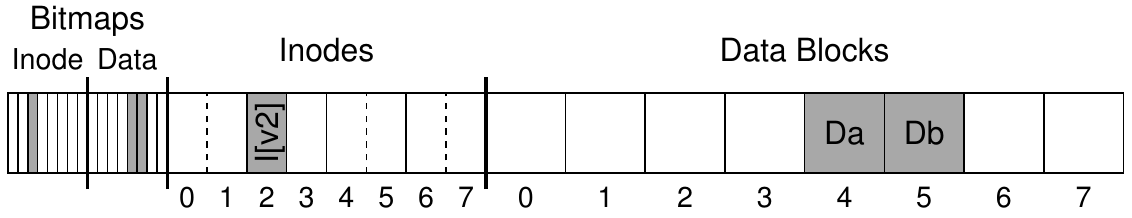
\includegraphics[width=1.\textwidth]{crash-ex-ver2}
			
			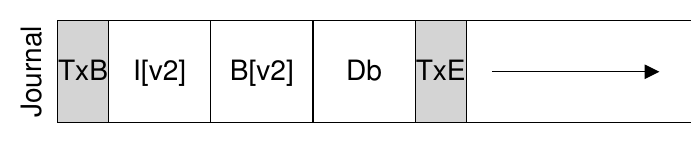
\includegraphics[width=1.\textwidth]{ext3-journal-struct}	
		\end{column}
		%		\pause
		\begin{column}{.5\textwidth}			
			方法2 : Data Journaling
			\begin{itemize}
				\item TxB:transaction 开始
				\item TxE:transaction 结束
				\item logical logging:中间3块数据
			\end{itemize}
			\pause
			上述transaction写到磁盘上后,更新磁盘,覆盖相关结构(checkpoint)
			\begin{itemize}	
				\item I[V2]
				\item B[v2]
				\item Db
			\end{itemize}
			
		\end{column}
	\end{columns}
	
\end{frame}
%----------------------------------------------
\begin{frame}[fragile]
	\frametitle{细节 -- 支持恢复异常 -- Data Journaling}
	%    \framesubtitle{xxxx}
	% from https://opensource.com/article/17/5/introduction-ext4-filesystem
	%		\centering
	%	\Large
	\begin{columns}
		\begin{column}{.5\textwidth}
			EXT4: 恢复异常文件系统 for crash-consistency problem
%			\centering
%			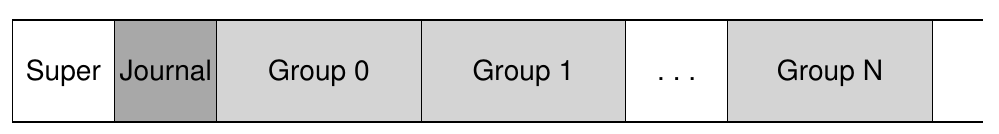
\includegraphics[width=1.\textwidth]{ext3-journal}
%			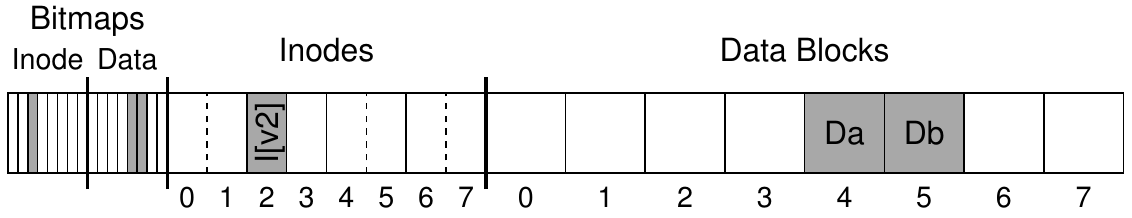
\includegraphics[width=1.\textwidth]{crash-ex-ver2}
			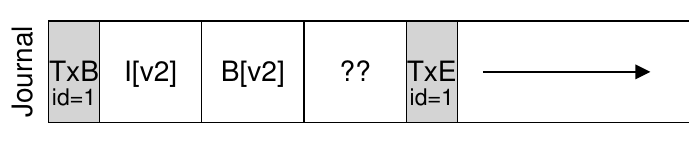
\includegraphics[width=1.\textwidth]{ext3-journal-struct-err}
			\pause
			\includegraphics[width=1.\textwidth]{ext3-journal-write}
			\includegraphics[width=1.\textwidth]{ext3-journal-commit}
		\end{column}
		%		\pause
		\begin{column}{.5\textwidth}			
			方法2 : Data Journaling
			\begin{itemize}
				\item  Journal write
				\item  Journal commit
				\item  Checkpoint
			\end{itemize}
			\pause
			恢复(Recovery):在此更新序列期间的任何时间都可能发生崩溃。
			\begin{itemize}	
				\item 如果崩溃发生在将事务安全地写入日志之前
				\item 如果崩溃是在事务提交到日志之后但在检查点完成之前发生

			\end{itemize}
			\pause
			\Large 太多写,慢!
		\end{column}
	\end{columns}
	
\end{frame}

%----------------------------------------------
\begin{frame}[fragile]
	\frametitle{细节 -- 支持恢复异常 -- Data Journaling}
	%    \framesubtitle{xxxx}
	% from https://opensource.com/article/17/5/introduction-ext4-filesystem
	%		\centering
	%	\Large
	\begin{columns}
		\begin{column}{.5\textwidth}
			EXT4: 恢复异常文件系统 for crash-consistency problem
			%			\centering
			%			\includegraphics[width=1.\textwidth]{ext3-journal}
			%			\includegraphics[width=1.\textwidth]{crash-ex-ver2}
%			\includegraphics[width=1.\textwidth]{ext3-journal-struct-err}
%			\pause
			\includegraphics[width=1.\textwidth]{ext3-journal-commit}
			\includegraphics[width=1.\textwidth]{ext3-journal-batch}
			\includegraphics[width=1.\textwidth]{ext3-journal-superblock}
		\end{column}
		%		\pause
		\begin{column}{.5\textwidth}			
			方法2 : Data Journaling: 提高速度
			\begin{itemize}
				\item  批处理日志更新
				\item  使日志有限:循环日志
				\item 日志超级块 journal	superblock
			\end{itemize}
			\pause
			新的更新过程
			\begin{itemize}	
				\item Journal write
				\item Journal commit
				\item Checkpoint
				\item Free:一段时间后,通过更新日记帐超级块将交易记录标记为空闲
				
			\end{itemize}

		\end{column}
	\end{columns}
	
\end{frame}


%----------------------------------------------
\begin{frame}[fragile]
	\frametitle{细节 -- 支持恢复异常 -- Metadata Journaling}
	%    \framesubtitle{xxxx}
	% from https://opensource.com/article/17/5/introduction-ext4-filesystem
	%		\centering
	%	\Large
	\begin{columns}
		\begin{column}{.5\textwidth}
			EXT4: 恢复异常文件系统 for crash-consistency problem
			%			\centering
			%			\includegraphics[width=1.\textwidth]{ext3-journal}
			%			\includegraphics[width=1.\textwidth]{crash-ex-ver2}
			%			\includegraphics[width=1.\textwidth]{ext3-journal-struct-err}
			%			\pause
			\includegraphics[width=1.\textwidth]{ext3-journal-commit}
			\includegraphics[width=1.\textwidth]{ext3-journal-metadata}
			\includegraphics[width=1.\textwidth]{ext3-journal-batch}
			\includegraphics[width=1.\textwidth]{ext3-journal-superblock}
		\end{column}
		%		\pause
		\begin{column}{.5\textwidth}			
			方法2 : Metadata Journaling: 进一步提高速度
			\begin{itemize}
				\item  我们什么时候应该将数据块Db写入磁盘? \pause
				\item 事实证明,数据写入的顺序对于仅元数据的日记记录确实很重要。
				\item  如果在事务(包含I [v2]和B [v2])完成后将 Db写入磁盘,这样有问题吗?
			\end{itemize}
%			\pause
%			新的更新过程
%			\begin{itemize}	
%				\item Data write
%				\item Journal metadata write
%				\item Journal commit
%				\item Checkpoint metadata
%				\item Free
%				
%			\end{itemize}
%			通过强制首先写入数据,文件系统可以保证指针永远不会指向垃圾数据。
		\end{column}
	\end{columns}
	
\end{frame}


%----------------------------------------------
\begin{frame}[fragile]
	\frametitle{细节 -- 支持恢复异常 -- Metadata Journaling}
	%    \framesubtitle{xxxx}
	% from https://opensource.com/article/17/5/introduction-ext4-filesystem
	%		\centering
	%	\Large
	\begin{columns}
		\begin{column}{.5\textwidth}
			EXT4: 恢复异常文件系统 for crash-consistency problem
			%			\centering
			%			\includegraphics[width=1.\textwidth]{ext3-journal}
			%			\includegraphics[width=1.\textwidth]{crash-ex-ver2}
			%			\includegraphics[width=1.\textwidth]{ext3-journal-struct-err}
			%			\pause
			\includegraphics[width=1.\textwidth]{ext3-journal-commit}
			\includegraphics[width=1.\textwidth]{ext3-journal-metadata}
			\includegraphics[width=1.\textwidth]{ext3-journal-batch}
			\includegraphics[width=1.\textwidth]{ext3-journal-superblock}
		\end{column}
		%		\pause
		\begin{column}{.5\textwidth}			
			方法2 : Metadata Journaling: 进一步提高速度 \\
%			\begin{itemize}
%				\item  我们什么时候应该将数据块Db写入磁盘? \pause
%				\item 事实证明,数据写入的顺序对于仅元数据的日记记录确实很重要。
%				\item  如果在事务(包含I [v2]和B [v2])完成后将 Db写入磁盘,这样有问题吗?
%			\end{itemize}
%			\pause
			新的更新过程
			\begin{itemize}	
				\item Data write
				\item Journal metadata write
				\item Journal commit
				\item Checkpoint metadata
				\item Free
				
			\end{itemize}
			通过强制首先写入数据,文件系统可以保证指针永远不会指向垃圾数据。
		\end{column}
	\end{columns}
	
\end{frame}



%----------------------------------------------
\begin{frame}[fragile]
	\frametitle{细节 -- 支持恢复异常 -- Metadata Journaling}
	%    \framesubtitle{xxxx}
	% from https://opensource.com/article/17/5/introduction-ext4-filesystem
	%		\centering
	%	\Large
	\begin{columns}[t]
		\begin{column}{.5\textwidth}
			\centering
			Data Journaling时间线
			\includegraphics[width=1.\textwidth]{ext3-journal-data-timeline}


		\end{column}
		%		\pause
		\begin{column}{.5\textwidth}	
			\centering
			Metadata Journaling时间线		
			\includegraphics[width=1.\textwidth]{ext3-journal-metadata-timeline}
		\end{column}
	\end{columns}
	
\end{frame}
%----------------------------------------------
\end{document}
